%%%%%%%%%%%%%%%%%%%%%%%%%%%%%%%%%%%%%%%%%%%%%%%%%%%%%%%%%%%%%%%%%%%%%%%%%%%
%% This file is part of the book
%%
%% Algorithmic Graph Theory
%% http://code.google.com/p/graph-theory-algorithms-book/
%%
%% Copyright (C) 2009, 2010, 2011 Minh Van Nguyen <nguyenminh2@gmail.com>
%%
%% See the file COPYING for copying conditions.
%%%%%%%%%%%%%%%%%%%%%%%%%%%%%%%%%%%%%%%%%%%%%%%%%%%%%%%%%%%%%%%%%%%%%%%%%%%

\tikzset{every mark/.append style={scale=0.5}}
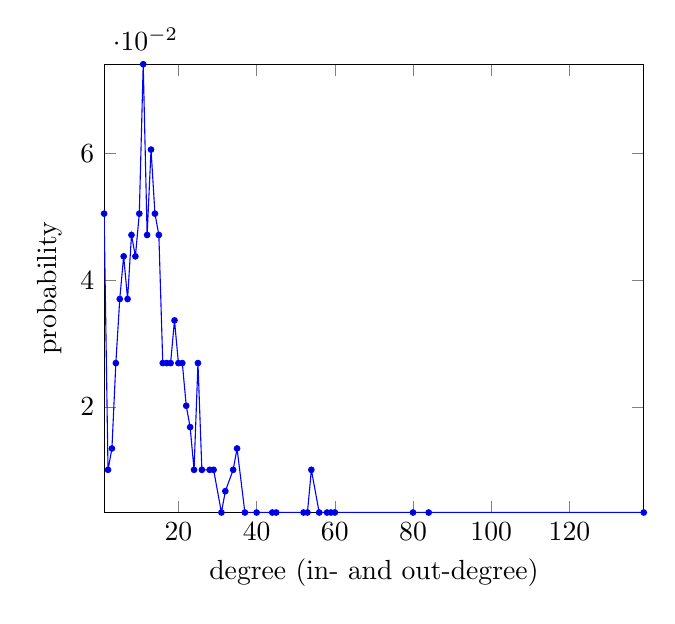
\begin{tikzpicture}[scale=1]
\begin{axis}[%
  enlargelimits=false,%
  xlabel=\text{degree (in- and out-degree)},%
  ylabel=\text{probability}%
]
\addplot+[sharp plot] coordinates
{
  (1, 0.0505050505050505)    (2, 0.0101010101010101)
  (3, 0.0134680134680135)    (4, 0.0269360269360269)
  (5, 0.0370370370370370)    (6, 0.0437710437710438)
  (7, 0.0370370370370370)    (8, 0.0471380471380471)
  (9, 0.0437710437710438)    (10, 0.0505050505050505)
  (11, 0.0740740740740741)   (12, 0.0471380471380471)
  (13, 0.0606060606060606)   (14, 0.0505050505050505)
  (15, 0.0471380471380471)   (16, 0.0269360269360269)
  (17, 0.0269360269360269)   (18, 0.0269360269360269)
  (19, 0.0336700336700337)   (20, 0.0269360269360269)
  (21, 0.0269360269360269)   (22, 0.0202020202020202)
  (23, 0.0168350168350168)   (24, 0.0101010101010101)
  (25, 0.0269360269360269)   (26, 0.0101010101010101)
  (28, 0.0101010101010101)   (29, 0.0101010101010101)
  (31, 0.00336700336700337)  (32, 0.00673400673400673)
  (34, 0.0101010101010101)   (35, 0.0134680134680135)
  (37, 0.00336700336700337)  (40, 0.00336700336700337)
  (44, 0.00336700336700337)  (45, 0.00336700336700337)
  (52, 0.00336700336700337)  (53, 0.00336700336700337)
  (54, 0.0101010101010101)   (56, 0.00336700336700337)
  (58, 0.00336700336700337)  (59, 0.00336700336700337)
  (60, 0.00336700336700337)  (80, 0.00336700336700337)
  (84, 0.00336700336700337)  (139, 0.00336700336700337)
};
\end{axis}
\end{tikzpicture}
